% §V Experiments — offline battery. REWRITE 08-11 (RESULTS_LINEUP.md A1–A3, 보고 정책).
% 08-11 결정: best-only 보고 (균일 규칙, 서두 선언); 용어 naive policy. 09-14: fig:doseresponse = figs/dose_response.tex (pgfplots, 스크립트 생성).
% 08-12 압축 (사용자): bypass 소절 + Table I 삭제 (유지).
% 08-12 재구성 (사용자): ① 결과 제시 probe 순서 P1→P4 (P5는 §VI-B) ② 표/서사 분리 —
%   §V-A = naive vs conditioned 2행 표 (tab:probes), §V-B = ablation 컨트롤 2행 표
%   (tab:ablation; wrench-kept/shuffled + bypass·grounding-not-capacity 문단).
%   P1 수치 출처 (fromnaive 라운드, val ep0 — probe_film_authority.py 헤더의 "training data"는
%   stale 라벨): 0729_{fromnaive_best,mask0fn_main,v1_main}_std.txt COMMITTED-desc Δdz.
%   P1은 mm만 보고 (% 금지: P1 분모 −7.8mm/frame ≠ P2 분모 −1.7mm/frame — % 병렬 오독 유발).
% 가드레일: "naive는 force-blind" 금지 (transplant 105%); 캘리브레이션 라운드 간 % 직접
% 비교 금지; 인스턴스 공시는 §IV 각주 전담. 로봇 배포 ckpt = val-best (사용자 확인 08-11).
\section{Experiments}
\label{sec:offline}

\begin{table*}[!t]
\caption{Offline battery. Upper rows: the naive policy vs.\ the conditioned policy (FiLM,
ours). Lower rows: ablation controls with the same initialization and data and one
ingredient removed. Entries are the change in commanded descent caused by the intervention;
percentages are relative to the policy's own descent on the evaluated frames (\% own; none for
P1, whose frames differ). Press sim = the seal-never press simulation. The naive policy has no
\chat{} to force (---).}
\label{tab:probes}
\centering\setlength{\tabcolsep}{4.5pt}
\begin{tabular}{llrrrr}
\toprule
Policy & Force access & \multicolumn{1}{c}{\makecell{Forcing (P1)\\{\scriptsize mm/frame}}} & \multicolumn{1}{c}{\makecell{Transplant (P2)\\{\scriptsize mm/frame (\% own)}}} & \multicolumn{1}{c}{\makecell{Dose-response (P3), $8\rightarrow12$\,N\\{\scriptsize mm/frame (\% own)}}} & \multicolumn{1}{c}{\makecell{Press sim (P4)\\{\scriptsize max depth (mm)}}} \\
\midrule
naive VLA   & raw wrench               & ---                     & $+1.63$ (105\%)            & $+1.41\rightarrow+1.12$ (36$\rightarrow$28\%) $\downarrow$ & 14.9 \\
FiLM (ours) & masked, grounded \chat{} & $\mathbf{+0.9}$         & $+1.57$ (\phantom{1}94\%)  & $+1.20\rightarrow\mathbf{+4.40}$ (31$\rightarrow$\textbf{115\%}) $\uparrow$ & \textbf{9.8} \\
\midrule
FiLM, wrench kept            & raw + dead \chat{}  & $\phantom{+}0.0$ & $+1.68$ (111\%)           & $+1.57\rightarrow+1.12$ (42$\rightarrow$30\%) $\downarrow$ & 11.9 \\
FiLM, mask, shuffled \chat{} & ungrounded pathway  & $-0.2$           & $-0.06$ (\phantom{10}0\%) & $-0.06\rightarrow-0.11$ ($\approx$0\%) $\phantom{\downarrow}$ & \textbf{57.2} \\
\bottomrule
\end{tabular}
\end{table*}

The backbone throughout is SmolVLA~\cite{smolvla}, a compact open VLA chosen so that a matched
ablation---four policies from one initialization---and the continued-training runs are
affordable; Sec.~\ref{sec:offline-pi0} repeats the central result on the $3$B-class $\pi_0$.
The offline experiments compare four policies that start from the \emph{same} trained naive
checkpoint and continue training on the \emph{same} demonstrations: the naive policy itself,
the full recipe (the conditioned policy), and two controls that each remove one ingredient:
one keeps the raw wrench in the state alongside \chat{} (no mask), the other keeps the mask but
trains on \chat{} values shuffled across the batch, so \chat{} no longer tracks the measured
force (no grounding) (Sec.~\ref{sec:offline-quintuple}). Imitation error on
held-out episodes is indistinguishable across all four ($0.84$--$0.96$\,mm per step): on the
data manifold, these are the same policy. Every reported model is its validation-loss-selected
(\emph{best}) checkpoint---one uniform selection rule for all policies. This is the retrofit
setting of Sec.~\ref{sec:method-mask}: continued training ran for $20$k steps, validation loss
selects the conditioned policy's checkpoint at $2{,}500$ steps, and the monotone form reported
below persists to the final checkpoint ($+0.97\rightarrow+3.44$\,mm at $8\rightarrow12$\,N).

\subsection{The two policies under intervention}
\label{sec:offline-main}

Table~\ref{tab:probes} (upper rows) and Fig.~\ref{fig:doseresponse} give P1--P4 for the naive
and conditioned policies; the controls follow in Sec.~\ref{sec:offline-quintuple}.

\begin{figure}[t]
\centering
% AUTO-GENERATED by scripts/make_dose_response_pgf.py — do not edit.
% Data: LGES/vla_training/probes/0729_state_*_ramp{8,10,12}.txt, ALL-frames row.
\definecolor{figcond}{HTML}{0072B2}
\definecolor{fignaive}{HTML}{D55E00}
\definecolor{figkept}{HTML}{CC79A7}
\definecolor{figshuf}{HTML}{009E73}
\definecolor{figmuted}{HTML}{767676}
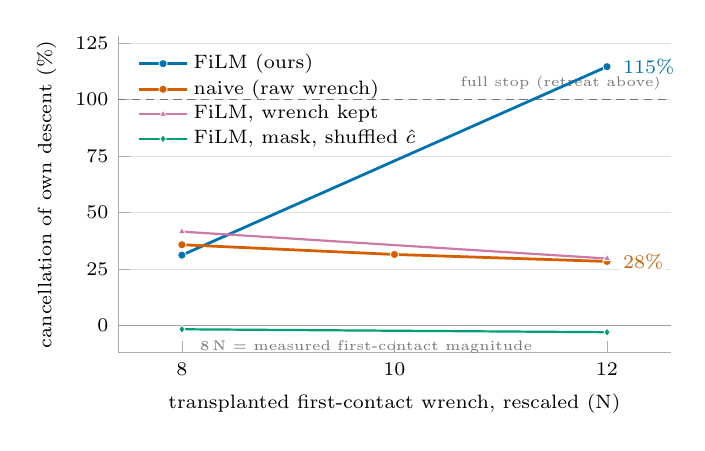
\begin{tikzpicture}
\begin{axis}[
  width=8.6cm, height=5.6cm, xmin=7.4, xmax=12.6, xtick={8,10,12},
  ymin=-12, ymax=128, ytick={0,25,50,75,100,125},
  xlabel={transplanted first-contact wrench, rescaled (N)},
  ylabel={cancellation of own descent (\%)},
  tick label style={font=\scriptsize}, label style={font=\scriptsize},
  axis x line*=bottom, axis y line*=left,
  axis line style={figmuted!60, line width=0.4pt},
  tick style={figmuted!60},
  ymajorgrids, grid style={figmuted!22, line width=0.3pt},
  clip=false, legend style={draw=none, fill=none, font=\scriptsize,
    legend cell align=left, at={(0.02,0.98)}, anchor=north west, row sep=-1.5pt},
]
\addplot[figmuted, dash pattern=on 3pt off 2pt, line width=0.5pt, forget plot] coordinates {(7.4,100) (12.6,100)};
\node[font=\tiny, figmuted, anchor=south east] at (axis cs:12.6,100) {full stop (retreat above)};
\addplot[figmuted!70, line width=0.4pt, forget plot] coordinates {(7.4,0) (12.6,0)};
\node[font=\tiny, figmuted, anchor=west] at (axis cs:8.08,-9.5) {8\,N = measured first-contact magnitude};
\addplot[figcond, solid, line width=1.0pt, mark=*, mark size=1.5pt, mark options={solid, fill=figcond, draw=white, line width=0.3pt}] coordinates {(8,31.2) (12,114.6)};
\addlegendentry{FiLM (ours)}
\node[font=\scriptsize, figcond, anchor=west, fill=white, inner sep=1pt] at (axis cs:12.12,114.6) {$115\%$};
\addplot[fignaive, solid, line width=1.0pt, mark=*, mark size=1.5pt, mark options={solid, fill=fignaive, draw=white, line width=0.3pt}] coordinates {(8,35.8) (10,31.5) (12,28.4)};
\addlegendentry{naive (raw wrench)}
\node[font=\scriptsize, fignaive, anchor=west, fill=white, inner sep=1pt] at (axis cs:12.12,28.4) {$28\%$};
\addplot[figkept, solid, line width=0.8pt, mark=triangle*, mark size=1.5pt, mark options={solid, fill=figkept, draw=white, line width=0.3pt}] coordinates {(8,41.6) (12,29.7)};
\addlegendentry{FiLM, wrench kept}
\addplot[figshuf, solid, line width=0.8pt, mark=diamond*, mark size=1.5pt, mark options={solid, fill=figshuf, draw=white, line width=0.3pt}] coordinates {(8,-1.6) (12,-2.9)};
\addlegendentry{FiLM, mask, shuffled $\hat{c}$}
\end{axis}
\end{tikzpicture}

% generated by scripts/make_dose_response_pgf.py from vla/probes/0729_state_*_ramp{8,10,12}.txt
\caption{Dose-response under forced wrench magnitude (P3): cancellation of each policy's
own commanded descent as the transplanted first-contact wrench is rescaled to
$8/10/12$\,N. The naive policy's response fades past the demonstrated range; the unmasked
variant lies on top of it (all response through the raw route); the ungrounded pathway is
flat at zero; only the grounded pathway grows with dose, crossing full cancellation into
commanded retreat at $12$\,N.}
\label{fig:doseresponse}
\end{figure}

\textbf{(P1) Condition forcing.} Forcing every channel of \chat{} to saturation moves the
conditioned policy's committed descent by $+0.9$\,mm per frame. Restricting the forcing to a
calibrated contact-onset pattern shows the limit of what any policy adopts: even the
best-conditioned policy moves by only $7\%$---the 1--2-frame contact \emph{transient} is
weakly adopted across the board.

\textbf{(P2) State transplant: both policies on one scale.}
\label{sec:offline-posthoc}
Transplanting a measured first-contact state into pre-contact descent frames moves the naive
policy by $+1.63$\,mm---$105\%$ of its descent command. The naive policy is not force-blind:
its raw route responds strongly to force-bearing state. In the conditioned policy the same
transplant acts entirely through \chat{} ($+1.57$\,mm, $94\%$): changing the wrench entries of
the state while holding \chat{} fixed moves the action by $0.00$\,mm---the mask leaves no
leak. \emph{Which} state is transplanted matters as
much as whether one is: a \emph{sealed} state (seal bit on, press wrench) brakes both policies
far more than a first-contact wrench does---in the on-robot probes of Sec.~\ref{sec:robot-live},
$147\%$ vs.\ $67\%$ of own descent for the naive policy and $58\%$ vs.\ $32\%$ for the
conditioned one. Together with
the weak contact-onset forcing above, the pattern is that stable, persistent conditions (seal,
sustained press) are adopted essentially for free, while a transient that is redundant with
depth-like cues in ordinary demonstrations is not; Sec.~\ref{sec:discussion} draws the
consequence for what mechanism can stop a stiff press.

\textbf{(P3) Dose-response: raw access binds a template, the grounded pathway binds a brake.}
The naive policy responds to transplanted force---at the demonstrated magnitude. As the dose
rises past the demonstrations, its response \emph{fades} ($36\%\rightarrow28\%$): a template,
matched ever more poorly as reality departs from it. The conditioned policy's response
\emph{grows} with dose, crossing full cancellation into commanded retreat at $12$\,N
($31\%\rightarrow115\%$)---where the unsaturated channel reads five times its training range.
The monotone extrapolation is not learned from data (no demonstration presses at these
forces); it is inherited from the channel's design as a calibrated monotone scalar. The forms
are not artifacts of checkpoint selection: no naive checkpoint we examined exceeds $65\%$
cancellation at any dose, while the grounded brake remains monotone to the end of training.
That the naive policy responds \emph{more} at the demonstrated dose does not help it: over-press
is the regime in which force rises past the template, so its brake weakens exactly as it becomes
necessary, and its strongest response---to the sealed state (Sec.~\ref{sec:robot-live})---is
bound to a signal that never arrives in an over-press.

\textbf{(P4) Press simulation: consequences.} Closing the loop under the seal-never press
turns the response forms into outcomes. Every conditioned episode settles by $9.8$\,mm of
penetration, with contact force at or below $7.1$\,N when the simulation ends. The naive
policy settles in four of six episodes but runs away in two---still descending when the step
budget ends, at up to $14.9$\,mm with force climbing through $13.1$\,N; its later checkpoints
respond \emph{more} in open loop yet fare \emph{worse} here ($3/6$, max $16.0$\,mm), because a
response that saturates below full cancellation cannot stop a stiff press regardless of its
size. The seal-granted control variant localizes the failure: given a seal event at shallow
depth the naive policy stops normally ($0.5$\,mm over-travel)---withhold the seal and it
presses through. Its stopping is real but bound to the \emph{seal event}; the conditioned
policy's is bound to \emph{force}.

\subsection{Ablating the recipe: the mask and the grounding}
\label{sec:offline-quintuple}

The two controls run the same battery (Table~\ref{tab:probes}, lower rows); each isolates one
ingredient.

\textbf{Remove the mask, and force reroutes: bypass.} The unmasked control keeps the raw
wrench in the state alongside \chat{}, and behaves as the naive policy everywhere: its
dose-response curve lies on top of the naive policy's ($+1.57\rightarrow+1.12$ vs.\
$+1.41\rightarrow+1.12$; identical at $12$\,N), forcing its \chat{} moves nothing ($0.0$\,mm),
and the pathway decomposition places its transplant response entirely on the raw route
($d_{\mathrm{FiLM}}{=}0.04$). With a redundant raw route available, gradient descent satisfies
the imitation objective through the already-functional path and starves the dedicated pathway.
This is the \emph{bypass} of Sec.~\ref{sec:intro}---and nothing in training registers it: the
unmasked variant's validation loss matches the conditioned policy's to the fourth decimal
($0.14750$ vs.\ $0.14762$). An independently trained pair under the earlier calibration
reproduces the result: $7\%$ condition-forcing authority with the wrench kept versus $76\%$
with it masked, again at near-identical loss.

\textbf{Remove the grounding, and the pathway is worse than raw access.} The shuffled control
has the same added parameters, the same continued training, the same pathway---and zero
response at every dose ($-0.2$\,mm under forcing; flat dose-response), with the worst
closed-loop outcome in the study: no episode settles, all six still descending at the step
budget, $19$--$23$\,N past the force limit, up to $57$\,mm deep. Grounding, not capacity,
is the active ingredient: the mask removed the raw route, and the noise-trained \chat{}
replaced it with nothing.

\subsection{The pathway attaches to a second backbone}
\label{sec:offline-pi0}
% 09-14 (사용자): π0 0729 film-state 결과 복원, π0.5 미언급. 출처 EXPERIMENTS_PI0_FILM_0729.md +
% probes/0729_sim_pi0{naive,filmstate,filmaction}_best_off1_fzdelta.txt, 0729_eval_pi0*, 0729_state_pi0filmstate_best_pc_fc.

The same pathway---same channels, same calibration, same mask---attaches to
$\pi_0$~\cite{pi0} ($3$B-class, ${\sim}8\times$ the parameter count) at its dense state token, with the
backbone otherwise unchanged. Fine-tuned naively on the same demonstrations, $\pi_0$
reproduces the naive failure: in the seal-never press no episode settles (mean penetration
$17.0$\,mm, max $19.6$). With the pathway attached, five of six settle (mean $7.2$\,mm) at equal
imitation error ($0.93$ vs.\ $1.03$\,mm per step), and the transplant response again runs
entirely through the FiLM route (masked raw route $+0.00$\,mm). Attaching the same pathway at
the \emph{action} token instead stops no episode ($22.9$\,mm mean): the injection site is part
of the recipe, not a detail.\footnote{This $\pi_0$ instance carries the saturating contact
channel but not the unsaturated $\chat_{\mathrm{fmag}}$, so its response is threshold-like
rather than dose-monotone, and one episode runs to $18.3$\,mm. Offline only; $\pi_0$ was not
deployed on the robot.}
